\section{eo\-VRPEdge\-Crossover Class Reference}
\label{classeo_v_r_p_edge_crossover}\index{eoVRPEdgeCrossover@{eoVRPEdgeCrossover}}
Implementation of the classic Edge Crossover from the TSP.  


{\tt \#include $<$eo\-VRPQuad\-Crossover.h$>$}

Inheritance diagram for eo\-VRPEdge\-Crossover::\begin{figure}[H]
\begin{center}
\leavevmode
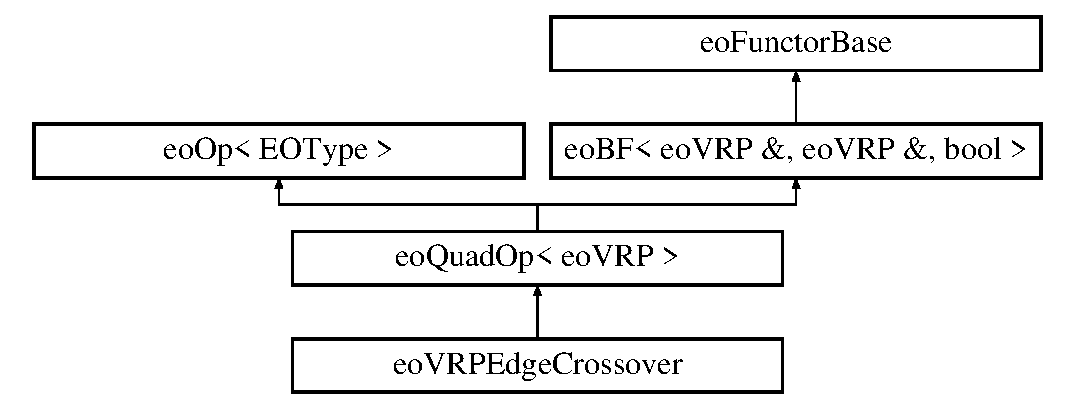
\includegraphics[height=4cm]{classeo_v_r_p_edge_crossover}
\end{center}
\end{figure}
\subsection*{Public Member Functions}
\begin{CompactItemize}
\item 
\bf{eo\-VRPEdge\-Crossover} ()\label{classeo_v_r_p_edge_crossover_1cec73fc43837a61b6c97812dd57891b}

\begin{CompactList}\small\item\em Deafult constructor. \item\end{CompactList}\item 
std::string \bf{class\-Name} () const 
\begin{CompactList}\small\item\em Returns a string containing the name of the class. \item\end{CompactList}\item 
bool \bf{operator()} (\bf{eo\-VRP} \&\_\-genotype1, \bf{eo\-VRP} \&\_\-genotype2)
\begin{CompactList}\small\item\em Both parameters are the parents and the (future) children of the crossover. \item\end{CompactList}\end{CompactItemize}
\subsection*{Private Member Functions}
\begin{CompactItemize}
\item 
bool \bf{Edge\-Crossover} (\bf{eo\-VRP} \&\_\-genotype1, \bf{eo\-VRP} \&\_\-genotype2, \bf{eo\-VRP} \&\_\-child)
\begin{CompactList}\small\item\em Actually performs the edge crossover. \item\end{CompactList}\item 
void \bf{remove\_\-entry} (unsigned \_\-vertex, std::vector$<$ std::set$<$ unsigned $>$ $>$ \&\_\-map)
\begin{CompactList}\small\item\em Removes a vertex from all his neighbours. \item\end{CompactList}\item 
void \bf{add\_\-vertex} (unsigned \_\-vertex, std::vector$<$ bool $>$ \&\_\-visited, std::vector$<$ std::set$<$ unsigned $>$ $>$ \&\_\-map, \bf{eo\-VRP} \&\_\-child)
\begin{CompactList}\small\item\em Adds a vertex to a child and erases it from the list of available vertices. \item\end{CompactList}\end{CompactItemize}


\subsection{Detailed Description}
Implementation of the classic Edge Crossover from the TSP. 



Definition at line 240 of file eo\-VRPQuad\-Crossover.h.

\subsection{Member Function Documentation}
\index{eoVRPEdgeCrossover@{eo\-VRPEdge\-Crossover}!className@{className}}
\index{className@{className}!eoVRPEdgeCrossover@{eo\-VRPEdge\-Crossover}}
\subsubsection{\setlength{\rightskip}{0pt plus 5cm}std::string eo\-VRPEdge\-Crossover::class\-Name (void) const\hspace{0.3cm}{\tt  [inline, virtual]}}\label{classeo_v_r_p_edge_crossover_8b2a199b70442852f93b2a34a42cf1e4}


Returns a string containing the name of the class. 

Used to display statistics. \begin{Desc}
\item[Returns:]The string containing the name of the class. \end{Desc}


Reimplemented from \bf{eo\-Quad\-Op$<$ eo\-VRP $>$}.

Definition at line 258 of file eo\-VRPQuad\-Crossover.h.\index{eoVRPEdgeCrossover@{eo\-VRPEdge\-Crossover}!operator()@{operator()}}
\index{operator()@{operator()}!eoVRPEdgeCrossover@{eo\-VRPEdge\-Crossover}}
\subsubsection{\setlength{\rightskip}{0pt plus 5cm}bool eo\-VRPEdge\-Crossover::operator() (\bf{eo\-VRP} \& {\em \_\-genotype1}, \bf{eo\-VRP} \& {\em \_\-genotype2})\hspace{0.3cm}{\tt  [inline, virtual]}}\label{classeo_v_r_p_edge_crossover_518856969ec708a73e728d36ddf01d1b}


Both parameters are the parents and the (future) children of the crossover. 

\begin{Desc}
\item[Parameters:]
\begin{description}
\item[{\em \_\-genotype1}]The first parent. \item[{\em \_\-genotype2}]The second parent. \end{description}
\end{Desc}
\begin{Desc}
\item[Returns:]True if any of the parents was modified. False otherwise. \end{Desc}


Implements \bf{eo\-BF$<$ eo\-VRP \&, eo\-VRP \&, bool $>$}.

Definition at line 272 of file eo\-VRPQuad\-Crossover.h.

References eo\-VRP::clean(), and Edge\-Crossover().\index{eoVRPEdgeCrossover@{eo\-VRPEdge\-Crossover}!EdgeCrossover@{EdgeCrossover}}
\index{EdgeCrossover@{EdgeCrossover}!eoVRPEdgeCrossover@{eo\-VRPEdge\-Crossover}}
\subsubsection{\setlength{\rightskip}{0pt plus 5cm}bool eo\-VRPEdge\-Crossover::Edge\-Crossover (\bf{eo\-VRP} \& {\em \_\-genotype1}, \bf{eo\-VRP} \& {\em \_\-genotype2}, \bf{eo\-VRP} \& {\em \_\-child})\hspace{0.3cm}{\tt  [inline, private]}}\label{classeo_v_r_p_edge_crossover_389bd29cab9e12915d0d5c4af80343d7}


Actually performs the edge crossover. 

\begin{Desc}
\item[Parameters:]
\begin{description}
\item[{\em \_\-genotype1}]First parent. \item[{\em \_\-genotype2}]Second parent. \item[{\em \_\-child}]Child. \end{description}
\end{Desc}
\begin{Desc}
\item[Returns:]True if the second parent was modified. False otherwise. \end{Desc}


Definition at line 301 of file eo\-VRPQuad\-Crossover.h.

References add\_\-vertex(), and eo\-Rng::random().

Referenced by operator()().\index{eoVRPEdgeCrossover@{eo\-VRPEdge\-Crossover}!remove_entry@{remove\_\-entry}}
\index{remove_entry@{remove\_\-entry}!eoVRPEdgeCrossover@{eo\-VRPEdge\-Crossover}}
\subsubsection{\setlength{\rightskip}{0pt plus 5cm}void eo\-VRPEdge\-Crossover::remove\_\-entry (unsigned {\em \_\-vertex}, std::vector$<$ std::set$<$ unsigned $>$ $>$ \& {\em \_\-map})\hspace{0.3cm}{\tt  [inline, private]}}\label{classeo_v_r_p_edge_crossover_df9886f80565a966c78fb5a08e12631f}


Removes a vertex from all his neighbours. 

\begin{Desc}
\item[Parameters:]
\begin{description}
\item[{\em \_\-vertex}]The vertex being erased. \item[{\em \_\-map}]The structure containing the neighbourhood relationship. \end{description}
\end{Desc}


Definition at line 380 of file eo\-VRPQuad\-Crossover.h.

Referenced by add\_\-vertex().\index{eoVRPEdgeCrossover@{eo\-VRPEdge\-Crossover}!add_vertex@{add\_\-vertex}}
\index{add_vertex@{add\_\-vertex}!eoVRPEdgeCrossover@{eo\-VRPEdge\-Crossover}}
\subsubsection{\setlength{\rightskip}{0pt plus 5cm}void eo\-VRPEdge\-Crossover::add\_\-vertex (unsigned {\em \_\-vertex}, std::vector$<$ bool $>$ \& {\em \_\-visited}, std::vector$<$ std::set$<$ unsigned $>$ $>$ \& {\em \_\-map}, \bf{eo\-VRP} \& {\em \_\-child})\hspace{0.3cm}{\tt  [inline, private]}}\label{classeo_v_r_p_edge_crossover_7917ea1dec6221f71127c6fae9515e68}


Adds a vertex to a child and erases it from the list of available vertices. 

\begin{Desc}
\item[Parameters:]
\begin{description}
\item[{\em \_\-vertex}]The vertex being added to the child. \item[{\em \_\-visited}]The vector of visited vertices. \item[{\em \_\-map}]The structure containing the neighbourhood relationship. \item[{\em \_\-child}]The child where we add the vertex. \end{description}
\end{Desc}


Definition at line 398 of file eo\-VRPQuad\-Crossover.h.

References remove\_\-entry().

Referenced by Edge\-Crossover().

The documentation for this class was generated from the following file:\begin{CompactItemize}
\item 
eo\-VRPQuad\-Crossover.h\end{CompactItemize}
